\documentclass[12pt,letterpaper]{article}

\usepackage{caption} % for the figure captions
\usepackage[osf]{mathpazo} % a nicer font
% this is a package for the citation formats: found this formulation sorted natbib errors when changing packages
%from http://tex.stackexchange.com/questions/54480/package-natbib-error-bibliography-not-compatible-with-author-year-citations
\usepackage[square,sort,comma,numbers]{natbib} 
\usepackage{amsmath} % package for equations
\usepackage{url} % package for urls
\usepackage{hyperref} % for hyperlinks
\usepackage[a4paper, total={6in, 9in}]{geometry}
\hypersetup{
     colorlinks   = true,
     citecolor    = gray
}
\usepackage{graphicx} % for the figures
\usepackage{pdfpages}

\hypersetup{linkcolor=blue}

\pagenumbering{gobble}

\graphicspath{ }

\begin{document}

%title

{\Huge\textbf{\textit{Dipterus}}\par}
\vspace{3mm}
{\large{Dip-ter-russ} \par} 
\vspace{5mm}
\textit{Dipterus} is a \textbf{lungfish} from the Devonian (420 to 360 million years ago) of Scotland - this makes it a \textbf{lobe-finned fish}, a group which also includes \textit{Osteolepis}.  There are only \textbf{three species of lungfish left alive today}: one each living in South America, Africa, and Australia, all of which have big crushing teeth for eating hard shelled prey. In the Devonian however lungfishes came in \textbf{far many more shapes and sizes}, including pike-like predators with sharp teeth!

\begin{figure}[h!]
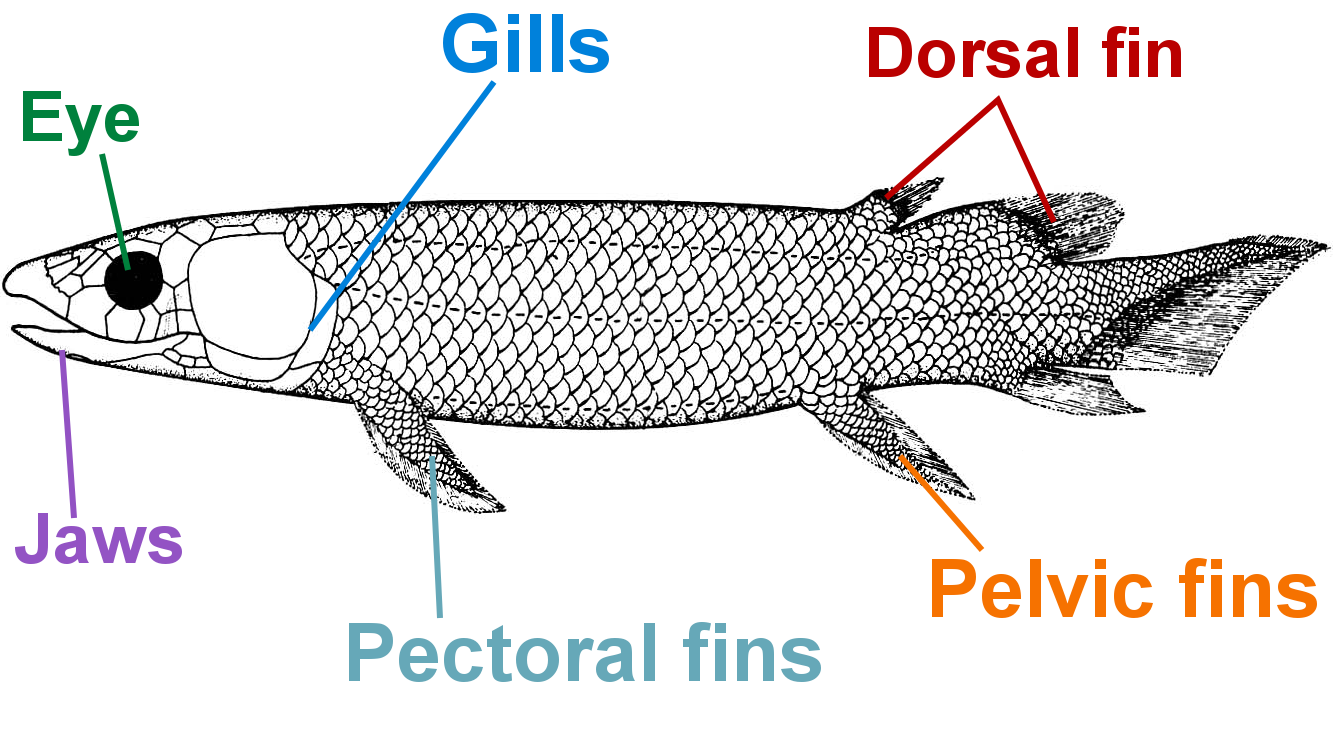
\includegraphics[scale=1.2]{Dipterus}
\centering
\end{figure}

{\large\textbf{\underline{Fossil facts}}\par}

\begin{itemize}
  \item As well as taking oxygen from water with their gills like other fishes, living lungfish are able to breathe air like land vertebrates (this is why they are called lungfish).  \textit{Dipterus} could probably do the same.
  \item Living lungfishes are also odd in that they can aestivate when the water they live in dries up: this means that they dig a hole and seal themselves in, shutting their body down until the water comes back.  We don't know if \textit{Dipterus} could do this.
\end{itemize}


\end{document}